\documentclass[pdftex]{beamer} 
% \usepackage[pdftex]{graphicx}
\usepackage{amsmath,amssymb,amsthm} 
\usepackage{pb-diagram}
% \usepackage[authoryear]{natbib}
% \bibliographystyle{plainnat}
% \setcitestyle{square,aysep={}}
\usepackage{pb-diagram}
\usepackage{ucs}
\usepackage[utf8x]{inputenc}
% \usepackage[russian]{babel}
\usepackage{epstopdf}
\usepackage{multicol}
\usepackage{cancel}

\usepackage{amsfonts}

%%%%%%%%%%%%%%%%%%%%%%%%%%%%%%%%%%%%%%%%%%%%%%%%%%%%%%%%%%%%%%%%%%%%%%%%%%%%%%%%%%%%%%%%%%%%%%%%%%% 

% \newtheorem{theorem}{Theorem}
%% \newtheorem{acknowledgement}[theorem]{Acknowledgement}
%% \newtheorem{algorithm}[theorem]{Algorithm}
%% \newtheorem{axiom}[theorem]{Axiom}
%% \newtheorem{case}[theorem]{Case}
%% \newtheorem{claim}[theorem]{Claim}
%% \newtheorem{conclusion}[theorem]{Conclusion}
%% \newtheorem{condition}[theorem]{Condition}
%% \newtheorem{conjecture}[theorem]{Conjecture}
%% \newtheorem{mycorollary}[theorem]{Corollary}
%% \newtheorem{mycriterion}[theorem]{Criterion}
%% \newtheorem{mydefinition}[theorem]{Definition}
%% \newtheorem{myexample}[theorem]{Example}
%% \newtheorem{myexercise}[theorem]{Exercise}
%% \newtheorem{mylemma}[theorem]{Lemma}
%% \newtheorem{mynotation}[theorem]{Notation}
%% \newtheorem{myproblem}[theorem]{Problem}
%% \newtheorem{myproposition}[theorem]{Proposition}
%% \newtheorem{myremark}[theorem]{Remark}
%% \newtheorem{mysolution}[theorem]{Solution}
%% \newtheorem{mysummary}[theorem]{Summary}
%% \newenvironment{myproof}[1][Proof]{\textbf{#1.} }{\ \rule{0.5em}{0.5em}}


\newcommand{\go}{\stackrel{\circ }{\mathfrak{g}}}
\newcommand{\ao}{\stackrel{\circ }{\mathfrak{a}}}
\newcommand{\co}[1]{\stackrel{\circ }{#1}}
\newcommand{\pia}{\pi_{\mathfrak{a}}}
\newcommand{\piab}{\pi_{\mathfrak{a}_{\bot}}}
\newcommand{\gf}{\mathfrak{g}}
\newcommand{\gfh}{\hat{\mathfrak{g}}}
\newcommand{\af}{\mathfrak{a}}
\newcommand{\afh}{\hat{\mathfrak{a}}}
\newcommand{\bff}{\mathfrak{b}}
\newcommand{\afb}{\mathfrak{a}_{\bot}}
\newcommand{\hf}{\mathfrak{h}}
\newcommand{\hfg}{\hf_{\gf}}
\newcommand{\hfb}{\mathfrak{h}_{\bot}}
\newcommand{\pf}{\mathfrak{p}}
\newcommand{\aft}{\widetilde{\mathfrak{a}}}

% \pagestyle{plain}

\theoremstyle{definition} \newtheorem{Def}{Definition}
\setbeamertemplate{caption}[empty]
\newcommand{\tr}{\hat\triangleright} \newcommand{\trc}{\triangleright}
\newcommand{\adk}{a^{\dagger}_{\kappa}} \newcommand{\ak}{a_{\kappa}}
\def\bF{\mbox{$\overline{\cal F}$}} \def\F{\mbox{$\cal F$}}

\usetheme{default}
% \usetheme{Warsaw}
\title[Tricritical Ising model]{Integrability and s-holomorphicity in tricritical Ising model}
\author[Anton Nazarov]{Anton Nazarov}

\institute[SPbSU]{
  Department of high-energy physics,\\
  Faculty of physics,\\ 
  Chebyshev laboratory,\\
  Faculty of mathematics and mechanics,\\
  Saint-Petersburg State University,\\
  198904, Saint-Petersburg, Russia\\
  e-mail: anton.nazarov@hep.phys.spbu.ru
}

\date[SQS'2013] % (optional, should be abbreviation of conference name)
{Supersymmetries and Quantum Symmetries 2013,\\ Joint Institute for Nuclear Research, Bogoliubov Laboratory of Theoretical Physics, July 31, 2013}

\begin{document}
\maketitle
\section{Introduction}
%% \begin{frame}
%%   \frametitle{Plan of the talk}
%%   \begin{itemize}
%%   \item Tricritical Ising model
%%   \item RSOS formulation and integrability
%%   \item CFT description and SLE 
%%   \item S-holomorphic observable
%%   \item Conclusion
%%   \end{itemize}
%% \end{frame}
\begin{frame}
  \frametitle{ Tricritical Ising model}
  Hamiltonian of the model
  \begin{equation}
    \label{eq:1}
    H = -\beta \sum_{<i,j>}\sigma_i\sigma_j - \mu \sum_{i}(\sigma_i)^2  
  \end{equation}
  Partition function
  \begin{equation}
    \label{eq:2}
    Z=\sum_{\mathrm{conf}} W[\mathrm{conf}]=\sum_{\mathrm{conf}} e^{-\frac{H[\mathrm{conf}]}{kT}}
  \end{equation}
  
  \begin{itemize}
  \item Conformal invariance in tricritical point
  \item Conformal field theory with $c=\frac{7}{10}$
  \item Supersymmetry, super-Virasoro algebra
  \item Integrability 
  \end{itemize}
\end{frame}

\section{RSOS models and integrability}

\begin{frame}
  \frametitle{$A_4$  restricted solid-on-solid model}
  Dynkin diagram, nodes: $1,\dots,4$, adjacent nodes -- adjacent values
  \begin{equation}
    \label{eq:4}
    A_4:\quad
    \begin{diagram}
      \node{1}\arrow{e,-}\node{2}\arrow{e,-}\node{3}\arrow{e,-}\node{4}
    \end{diagram}
  \end{equation}

  \begin{equation}
    \label{eq:3}
    W[\mathrm{conf}]=\prod_{\mathrm{faces}} W(\mathrm{face}) =\prod W\left(\left.\begin{array}{cc}d & c\\a &b\end{array} \right| \lambda, u\right)
  \end{equation}
  $2\cos(\lambda)$ -- highest eigenvalue of the adjacency matrix, $\psi$ -- eigenvector, $u$ -- spectral parameter.

Bolzmann weight for a face with vertex labels $a,b,c,d$ is 
\begin{equation}
    W\left.\left(
    \begin{array}{cc}
      d & c\\
      a & b
    \end{array}\right| u \right)
= \frac{\sin(\lambda-u)}{\sin\lambda}\delta_{ac} + \frac{\sin(u)}{\sin\lambda}\frac{ \psi_a^{1/2}
  \psi_c^{1/2}}{\psi_b} \delta_{bd},
\end{equation}
Boltzmann weights satisfy Yang-Baxter equation:
\begin{multline}
  \label{eq:15}
  \sum_{g} W\left.\left(
    \begin{array}{cc}
      f & g\\
      a & b
    \end{array}\right| u-v \right) W\left.\left(
    \begin{array}{cc}
      g & d\\
      a & b
    \end{array}\right| u \right) W\left.\left(
    \begin{array}{cc}
      f & e\\
      g & d
    \end{array}\right| v \right)=\\
  \sum_{g} W\left.\left(
    \begin{array}{cc}
      a & g\\
      b & c
    \end{array}\right| v \right) W\left.\left(
    \begin{array}{cc}
      f & e\\
      a & g
    \end{array}\right| u \right) W\left.\left(
    \begin{array}{cc}
      e & d\\
      g & c
    \end{array}\right| u-v \right)
\end{multline}
\end{frame}
\begin{frame}
  \frametitle{$A_4$ RSOS model weights at conformal point}
  \begin{equation}
    \label{eq:7}
    u=\lambda/2\quad \mbox{--\quad conformal point}
  \end{equation}

  \begin{equation}
    \label{eq:8}
    \lambda = \frac{\pi}{5}, \quad u=\frac{\pi}{10}
  \end{equation}

  After proper normalization we have
  \begin{equation}
    \label{eq:12}
    \begin{array}{l}
      W\left(                                          
        \begin{array}{cc}
          2 & 1 \\
          1 & 2
        \end{array}
      \right)=
      W\left(
        \begin{array}{cc}
          3 & 4 \\
          4 & 3
        \end{array}
      \right)=   W\left(                                         
        \begin{array}{cc}
          1 & 2 \\
          2 & 1
        \end{array}
      \right)= 
      W\left(                                                  
        \begin{array}{cc}
          4 & 3 \\
          3 & 4
        \end{array}
      \right)=\\\quad=\sqrt{\frac{2}{1+\sqrt{5}}}+\sqrt{\frac{1}{2}\left(1+\sqrt{5}\right)}\\
      W\left(                                      
        \begin{array}{cc}
          2 & 3 \\
          1 & 2
        \end{array}
      \right)=
      W\left(                                         
        \begin{array}{cc}
          3 & 2 \\
          4 & 3
        \end{array}
      \right)=    W\left(                                         
        \begin{array}{cc}
          3 & 4 \\
          2 & 3
        \end{array}
      \right)=    W\left(                                         
        \begin{array}{cc}
          2 & 1 \\
          3 & 2
        \end{array}
      \right)=\\
      W\left(                                       
        \begin{array}{cc}
          3 & 2 \\
          2 & 1
        \end{array}
      \right)=
      W\left(                                                       
        \begin{array}{cc}
          1 & 2 \\
          2 & 3
        \end{array}
      \right)=    W\left(                                                      
        \begin{array}{cc}
          4 & 3 \\
          3 & 2
        \end{array}
      \right)=
      W\left(                                                        
        \begin{array}{cc}
          2 & 3 \\
          3 & 4
        \end{array}
      \right)=\\
      \quad=\sqrt[4]{\frac{2}{1+\sqrt{5}}}\\
      W\left(
        \begin{array}{cc}
          3 & 2 \\
          2 & 3
        \end{array}
      \right)=    W\left(
        \begin{array}{cc}
          2 & 3 \\
          3 & 2
        \end{array}
      \right)=2 
    \end{array}
  \end{equation}
\end{frame}
\begin{frame}
  \frametitle{RSOS formulation and integrability}
  Consider model on a cylinder $N\times 2M$. 

  Double row transfer matrix:
  \begin{multline}
    \label{eq:5}
    D_N(u,\mbox{left boundary},\mbox{right boundary})=\sum_{c_0,\dots,c_N} B_{\mathrm{left}}(c_0,b_0,d_0| u)\cdot\\
    \cdot\prod_{j=0}^{N-1} W \left(\left.\begin{array}{cc} c_j & c_{j+1} \\ b_j & b_{j+1} \end{array}\right| u\right) 
    W \left(\left.\begin{array}{cc} d_j & d_{j+1} \\ c_j & c_{j+1} \end{array}\right| u\right) B_{\mathrm{right}} (c_N, b_N, d_N|u)
  \end{multline}
  Partition function is a sum of powers of eigenvalues
  \begin{equation}
    \label{eq:9}
    Z_{NM}(u)=\mathrm{tr} (D_N(u))^M=\sum_k \Lambda_N(u)_k ^M
  \end{equation}
  At conformal point $D_N$ is decomposed into a product of one-row transfer matrices. 
\end{frame}

\section{Conformal invariance and SLE}

\begin{frame}
  \frametitle{ Conformal field theory in critical limit }
  Take limit and obtain
  \begin{equation}
    \label{eq:10}
    Z_{r_1,a_1|r_2,a_2}(q) = \sum_{r=1}^{g-2} \sum_{s=1}^{g-1} F(A_{g-2})_{r_1,r_2}^r F({\cal G})_{a_1,a_2}^s \chi_{(r,s)}(q)
  \end{equation}
  Here $F(A_{g-2})_{r_1,r_2}^r$, $F({\cal G})_{a_1,a_2}^s$ are fused adjacency matrices,\\ $\chi_{(r,s)}(q)$ -- Virasoro characters for primary fields in minimal model
  \begin{equation}
    \label{eq:11}
    c=1-\frac{6}{g(g-1)}
  \end{equation}
  \begin{equation}
    \label{eq:13}
    \Delta_{(r,s)}=\frac{(rg-s(g-1))^2-1}{4g(g-1)}
  \end{equation}

  Problem: no connection with geometry, no explicit conformal invariance.
%%  $\Delta_{(r,s)}$, b.c.c., SLE, $\kappa$. 
\end{frame}
\begin{frame}
  \frametitle{Boundary conditions and Schramm-Loewner evolution}
  \begin{itemize}
  \item In critical point we expect conformal invariance.
  \item Use conformal maps to reference domain -- upper half plane. 
  \end{itemize}
  \begin{figure}[h]
    \begin{multicols}{2}

\begin{minipage}[h]{1.0\linewidth}
\vspace{-1cm}
\begin{equation*}
  \label{eq:13}
  \underline{\begin{array}{llllllllll}
    4 & & 4 &  & 2 &  & 2 &  & 2\\
    & 3 & & 3 & - & 3 & -  & 3 & & \\
    2 & & 2 & | & 4 &  & 4 & | & 2\\
    & 1 & & 3 & - & 3 &   & 3 & & \\
    2 & & 2 &  & 2 & | & 4 & | & 2\\
    & 1 & & 3 & - & 3 & & 3 &- & \\
    2 & & 2 & | & 4 & & 4 & & 4\\
    &  3 & & 3 &- & 3 &- & 3 &- &
  \end{array}}
\end{equation*}
\vspace{-0.7cm}
\caption{Domain wall in $A_{4}$ model}
\end{minipage}


      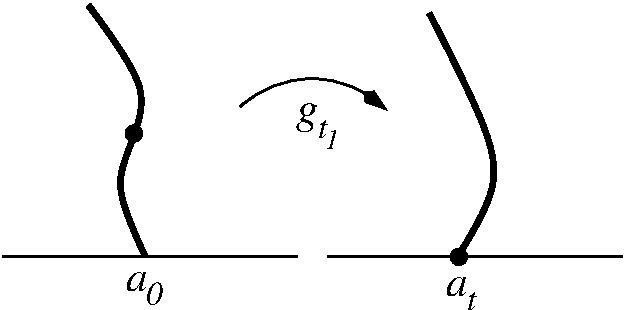
\includegraphics[width=50mm]{loewner.pdf}
      \caption{Conformal map}
      \label{fig:sle}
    \end{multicols}
  \end{figure}    
 \vspace{-0.7cm}
    {\it Schramm-Loewner evolution} on the upper half-plane $\mathbb{H}$ is a stochastic process which satisfies equation
    \begin{equation*}
      \frac{\partial g_t(z)}{\partial t} = \frac{ 2}{g_t(z)-\sqrt{\kappa}\xi_{t}}%% \quad \text{or} \quad       d w _{t}= \frac{2dt}{w_{t} }-\sqrt{\kappa}\xi_{t}
    \end{equation*}

  Conformally-invariant probability measure on trajectories $\gamma_{t}$ in $\mathbb{H}$.

\end{frame}
\begin{frame}
  \frametitle{SLE and boundary CFT}
  Boundary conditions correspond to boundary fields in CFT
  \begin{table}[h]
    \centering
    \begin{tabular}{|c|c|c|}
      \hline
      Symbol & Conformal weight &  Boundary condition\\
      \hline
&&\\
      $I$ & $0$ &
      $\underline{\begin{array}{llllllllll}
            2 & & 2 &  & 2 &  & 2 &  & 2\\
            & 1 & & 1 &  & 1 &   & 1 & & \\
          \end{array}}$\\

      $\varepsilon$ & $\frac{1}{10}$ &
      $\underline{\begin{array}{llllllllll}
            1 & & 1 &  & 3 &  & 3 &  & 1\\
            & 2 & & 2 &  & 2 &   & 2 & & \\
          \end{array}}$\\

      $\varepsilon'$ & $\frac{3}{5}$ &
      $\underline{\begin{array}{llllllllll}
            2 & & 4 &  & 4 &  & 2 &  & 4\\
            & 3 & & 3 &  & 3 &   & 3 & & \\
          \end{array}}$\\

      $\varepsilon''$ & $\frac{3}{2}$ &
      $\underline{\begin{array}{llllllllll}
            3 & & 3 &  & 3 &  & 3 &  & 3\\
            & 4 & & 4 &  & 4 &   & 4 & & \\
          \end{array}}$\\
      $\sigma'$ & $\frac{7}{16}$ &
      $\underline{\begin{array}{llllllllll}
            3 & & 3 &  & 3 &  & 3 &  & 3\\
            & 2 & & 2 &  & 2 &   & 2 & & \\
          \end{array}}$\\

      $\sigma$ & $\frac{3}{80}$ & free\\
&&\\
\hline
    \end{tabular}
%    \caption{Boundary conditions and boundary fields}
    \label{tab:bcc}
  \end{table}
  Change of boundary conditions $\leftrightarrow$ fusion rules for fields in CFT
\end{frame}
\begin{frame}
  \frametitle{ S-holomorphic observable}
  How to prove the convergence for correlation functions?

  Strategy employed for the Ising model:
  \begin{itemize}
  \item Introduce discrete holomorphic observables
  \item Solve boundary problem
  \item Prove the convergence in continuum limit
  \end{itemize}
  This strategy breaks for discrete holomorphic functions, since square is not discrete holomorphic. \\
  More strict condition is required $\Rightarrow$ $s$-holomorphicity.
%  Local conservation laws, discrete holomorphicity, continuation operator and transfer matrix
  \begin{figure}[h]
    \centering{
      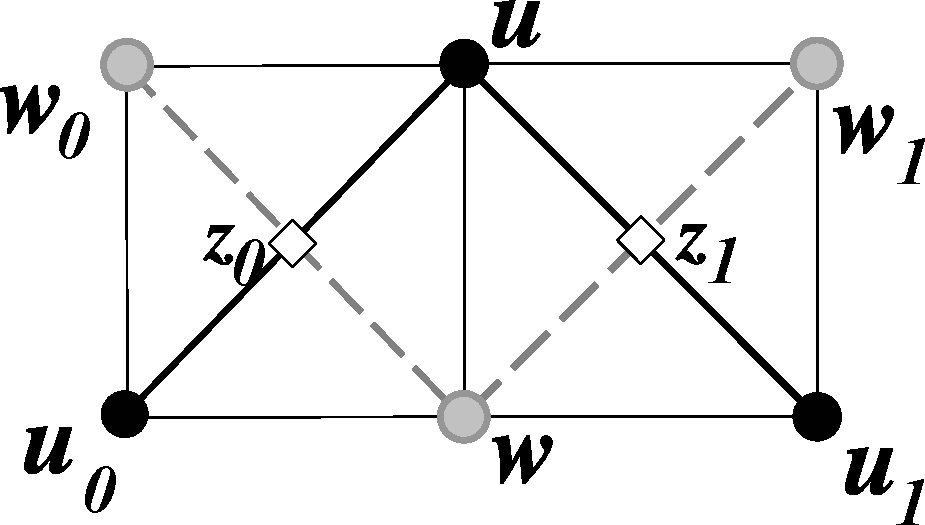
\includegraphics[height=25mm]{DefSHol}
    }
    \label{fig:phase-diagram}
  \end{figure}
  \begin{equation}
    \label{eq:14}
    \mathrm{Proj}\left[F(z_{0}), (i(w_{1}-u))^{-\frac{1}{2}}\right] = \mathrm{Proj}\left[F(z_{1}), (i(w_{1}-u))^{-\frac{1}{2}}\right] 
  \end{equation}
\end{frame}
\begin{frame}
  \frametitle{Candidate for $s$-holomorphic observable in $A_{4}$ RSOS model}
  \begin{equation}
    \label{eq:6}
    F(z)=\frac{1}{Z}\sum_{\substack{\mathrm{conf}:\\\gamma:a\to z}} \prod_{\mathrm{face}\in \gamma}W[\mathrm{face}] e^{-i s W(\gamma)}
  \end{equation}
  Here $W(\gamma)$ is winding number for the domain wall $\gamma:a\to z$. 

  Possible values for conformal weight $s$ are $\frac{1}{10}$, $\frac{7}{16}$. \\
  \vspace{1cm}
  Problem is to check that this observable solves boundary problem and prove the convergence. 
\end{frame}
\begin{frame}
  \frametitle{ Conclusion}
  \begin{itemize}
  \item Integrability can be used to get the structure of conformal field theory in critical point
  \item Conformal invariance is not manifest
  \item Discrete holomorphicity is required for the proof of correlation functions convergence
  \item $s$-holomorphicity is the consequence of the integrable choice of Boltzmann weights
  \end{itemize}
\end{frame}
\bibliography{bibliography}{} 
\bibliographystyle{apalike}
\end{document}
